Метод назван в честь французского математика Андре Сент-Лагю, хотя исторически эквивалентный метод был предложен сенатором Дэниэлом Вебстером для распределения мест в Конгрессе США \cite{balfair}. Он использует нечётные делители $1,3,5,\ldots$ и считается нейтральнее по отношению к размеру партий; в чистом виде он не даёт систематического преимущества ни крупным, ни мелким партиям \cite{gallprop}.

Алгоритм полностью аналогичен алгоритму метода Д'Ондта за исключением использования нечетных делителей:
\begin{equation*}
    D^{(k)}_i = \frac{V_i}{2s_i+1}
\end{equation*}

Например, если в выборах участовало 4 партии получившие соответственно 10000, 80000, 30000 и 20000 голосов, то распределение 8 мандатов для них будет выглядеть следующим образом:
\begin{center}
    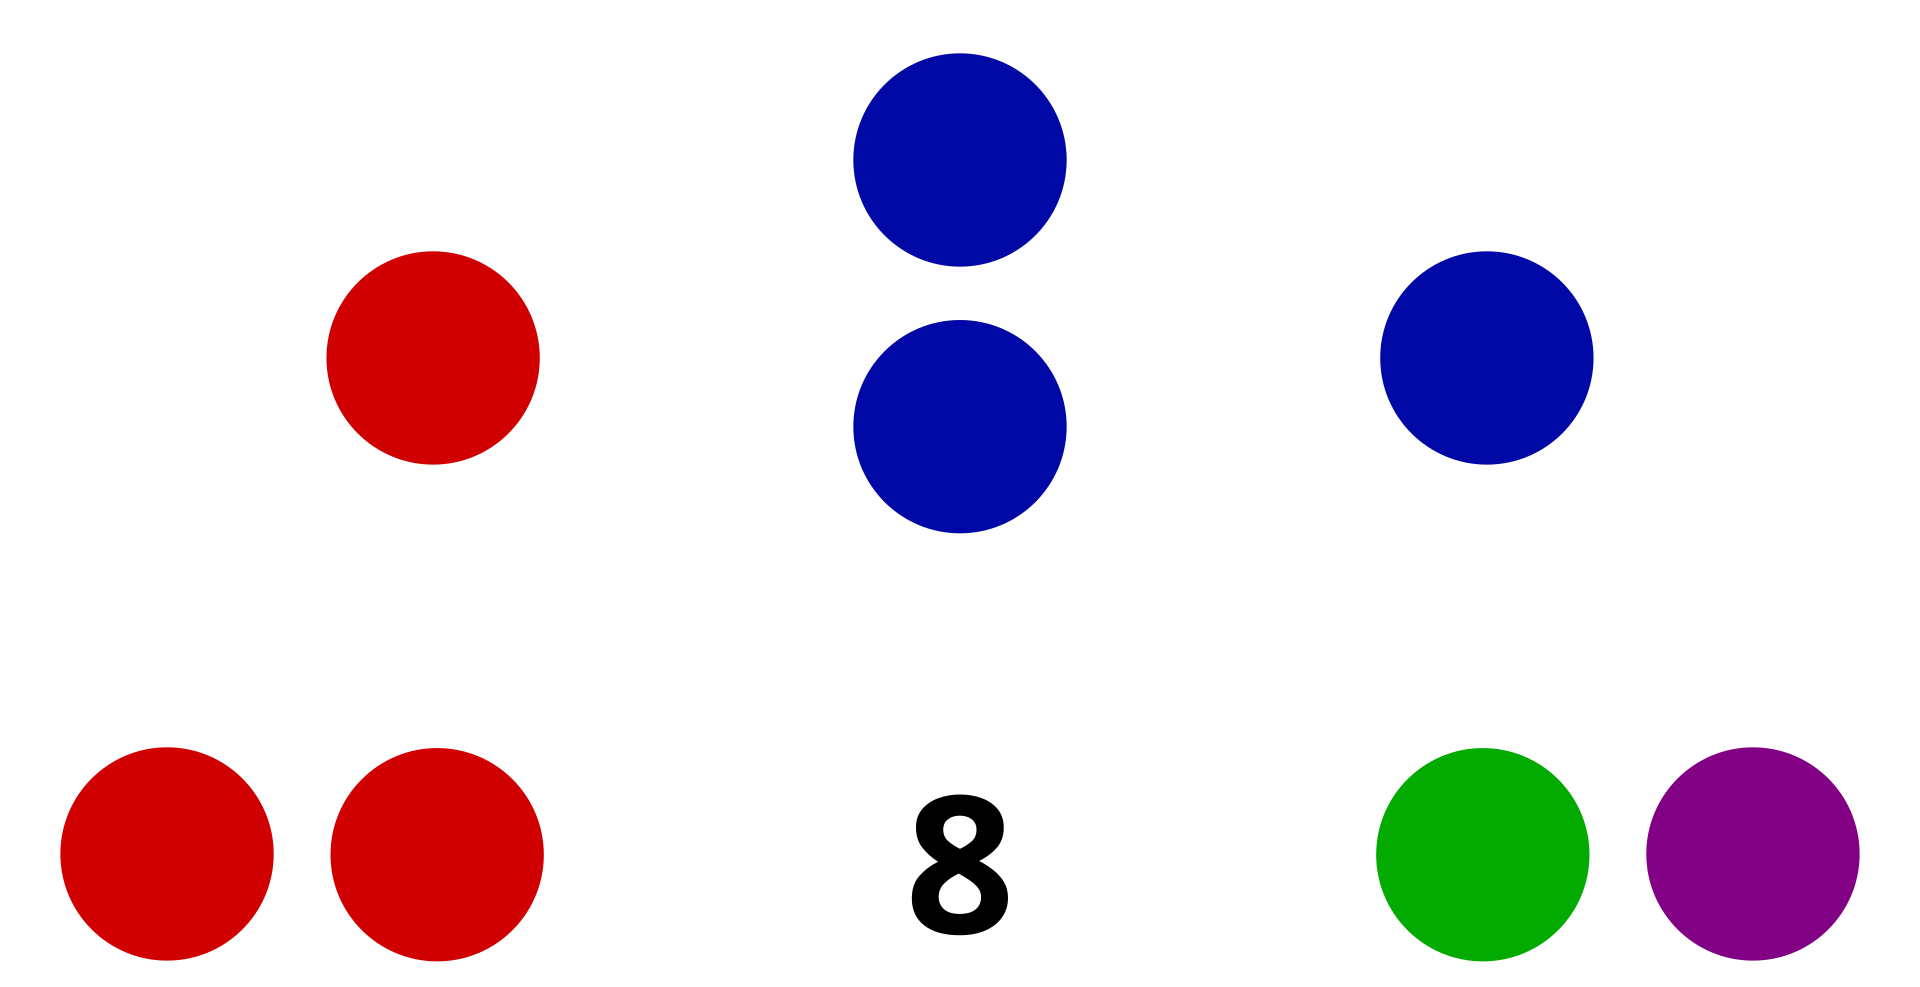
\includegraphics[width = 0.7\textwidth]{LaTeX/task3/img/sl.png}

    Рисунок 1. На Википедии лежат эти красивые png-шки, ну я их и использую
\end{center}
